\begin{center}	
\textbf{BOLETÍN DE EJERCICIOS 1}
\end{center}

\vspace{.2cm}

\begin{enumerate}[\bfseries \mbox{EJERCICIO} 1.]

    %---------- EJERCICIO 1 -----------------
    \item  Reproduzca para otros países diferentes a España el siguiente cuadro macroeconómico con datos 2021-2022.

    \begin{table}[htbp]
      \centering
      \caption{Escenario macroeconómico de Alemania (2021-2022)}
      \begin{center}
      Variación anual en $\%.$ A precios constantes.
      \end{center}
      \scalebox{0.5}{
	\begin{tabular}{l|r|r}
	\toprule
	      & \multicolumn{1}{l}{2021} & \multicolumn{1}{l}{2022} \\
	\midrule
	Gasto en consumo final nacional privado   & 0.4\%   & 4.5\% \\
	Gasto en consumo final de las AAPP & 3.8\%   & 2.2\% \\
	Formación bruta de capital fijo & 1.2\%   & 0.3\% \\
	\hspace{.3cm}Bienes de equipo y activos cultivados & 3.4\% & 2.2\% \\
	\hspace{.3cm}Construcción & 0\%   & -1.2\% \\
	Demanda Nacional (contribución al crecimiento del PIB) & -1.1\%  & 1.4\% \\
			Exportaciones de bienes y servicios&9.7\%&1.4\%\\
			   Importación de bienes y servicios&9\%&5\%\\
	   Saldo exterior (contribución al crecimiento del PIB)&0.7\%&-1.1\%\\
	   \textbf{PIB real} &2.6\%&1.5\%\\
	   Deflactor del PIB &3\%&5.3\%\\
	\bottomrule
	\end{tabular}%
	}
      \label{tab:addlabel}%
      \begin{center}
      \tiny Fuente: AMECO online.
      \end{center}
    \end{table}

    %---------- EJERCICIO 2 -----------------
    \item Reproduzca para otros países diferentes a España el siguiente cuadro macroeconómico.\\\\

    \begin{table}[htbp]
      \centering
      \caption{Los principales indicadores coyunturales de la economía Alemana}
      \begin{center}
      \scriptsize Variación en $\%$ respecto al mismo periodo del año anterior (precios constantes).
      \end{center}
      \vspace{0.3cm}
      \scalebox{0.5}{
	\begin{tabular}{l|l|c|c|c|rr|rrrr|rrrr}
	\toprule
	& Indicador & Unidad & Fuente &  Media 2000-2022 & 2021 & 2022 & I21 & II21 & III21 & IV21 & I22 & II22 & III22 & IV22\\
	\midrule
	    1.& PIB, pm&\%&Destatis&1.2&2.6&1.5&-2.3&10.6&1.8&1.2&3.9&1.7&1.3&0.3\\
	    1.b. &\quad PIB precios corrientes &MM EUR&Destatis&2782.1&3601.8&3867.1&862&878.1&916&945.7&939&948.6&972.2&1.007.3\\
	    2 &Demanda nacional (contrib. al crec. PIB en pp)&\%&Destatis&-0.12&-1.14&1.4&-4&7.3&1.2&1.3&5.5&3.2&1.5&0.1\\
	    3 &Saldo exterior (contrib. al crec. PIB en pp)&\%&Destatis&0.5&0.7&-1.1&1.2&3.8&-0.4&-1.2&-0.9&-1.8&-1.5&-0.6\\
	    4 &Gasto en consumo final hogares e ISFLSH &\%&Destatis&0.8&0.4&4.5&-8.7&6.5&1.4&3.1&8.5&7&2.1&0.4\\
	    5 &Gasto en consumo final AA.PP.&\%&Destatis&1.8&3.8&2.2&3.4&8.5&2.1&1.4&4.2&-0.1&0.2&0.5 \\
	    6 &Formación bruta de capital fijo&\%&Destatis&1&1.2&0.3&-1.1&8.7&0&-2.3&2.3&-1.3&2&-1.2\\
	    7 &\quad FBCF Construcción&\%&Destatis&-0.03&0&-1.2&-2.0&4.4&0.6&-3.2&3.4&-3.4&-1.7&-4.9\\
	    7.a. &\qquad FBCF Viviendas&\%&Destatis&-0.01&0.55&-2.2&-1.4&5.2&1.6&-3.4&3.4&-3.9&-2.3&-5.5\\
	    7.b. &\qquad FBCF otros edificios y estructuras&\%&Destatis&-0.02&-0.9&-1&-2.9&3.1&-1.1&-2.9&3.5&-2.6&-0.9&-3.8\\
	    8 &\quad FBCF bienes de equipo y activos cultivados e inmateriales&\%&Destatis&1.8&3.5&2.3&1.1&20.8&-2.1&-2.6&0.7&0.7&8.9&3.1\\
	    9 &Exportaciones de bienes y servicios&\%&Destatis&4.4&9.7&1.4&-0.2&28.2&7.4&7.2&3.6&2.4&5.1&0.5\\
	    10 &Importaciones de bienes y servicios&\%&Destatis&4&9&5&-2.9&20.6&9.3&11.1&6.3&6.9&9.2&1.9\\
	\bottomrule
	\end{tabular}%
      \label{tab:addlabel}%
	}
      \begin{center}
      \end{center}
    \end{table}


    %---------- EJERCICIO 3 -----------------
    \item Obtenga la aportación al crecimiento económico de los diferentes componentes del gasto en el país elegido por su grupo. Use datos de frecuencia anual para una muestra del 2000-2022.\\\\

    \begin{table}[htbp]
      \centering
      \caption{Contribución al crecimiento del PIB ajustado por precios, Alemania (\%)}
      \vspace{0.3cm}
      \scalebox{0.5}{
	\begin{tabular}{l|*{22}{r}}
	\toprule
	&2001&2002&2003&2004&2005&2006&2007&2008&2009&2010&2011&2012&2013&2014&2015&2016&2017&2018&2019&2020&2021&2022\\
	\midrule
	    Usos domesticos&0.2&-2.3&0.3&0.2&2.8&1.5&1&-3.1&3&3.1&-0.8&1&1.6&1.3&2.8&2.5&2.5&1.5&1.6&-2.9&1.8&2.9\\
	Gasto consumo final&0.8&-0.6&0.4&0.2&0.5&1&0.2&0.9&0.5&0.7&1.2&1.1&0.5&0.9&1.6&2.1&1.1&0.9&1.4&-2.1&1&2.4\\
	\qquad Gasto consumo final hogares&0.7&-0.8&0.2&0.4&0.4&0.8&-0.1&0.2&-0.1&0.4&1.0&0.8&0.2&0.6&1.0&1.3&0.8&0.8&0.9&-2.9&0.2&2.1\\
	\qquad Gasto consumo final AA.PP.&0.1&0.2&0.1&-0.1&0.1&0.2&0.3&0.7&0.6&0.3&0.2&0.2&0.3&0.3&0.6&0.8&0.3&0.2&0.5&0.8&0.8&0.3\\
	Formación bruta de capital fijo&-0.6&-1.3&-0.3&-0.1&0.2&1.4&0.7&0.3&-1.9&1.0&1.4&-0.1&-0.3&0.7&0.4&0.8&0.5&0.7&0.4&-0.5&0.3&0.1\\
	\qquad FBCF Equipos&0.8&-0.7&0&0.3&0.5&0.9&0.6&0.2&-1.6&0.7&0.5&-0.1&-0.2&0.3&0.3&0.2&0.3&0.3&0.1&-0.8&0.2&0.2\\
	\qquad FBCF Construcción&-0.5&-0.6&-0.2&-0.4&-0.3&0.4&0.0&-0.1&-0.3&0.3&0.8&0.1&-0.1&0.2&-0.1&0.4&0.1&0.3&0.1&0.4&0.0&-0.2\\
	Saldo exterior&1.5&2.1&-1&1.5&0.6&1.0&1.4&0.0&-2.6&1.2&0.8&1.3&-0.6&0.6&0.2&-0.6&0.2&-0.6&-0.6&-0.8&0.8&-1.2\\
	\qquad Exportaciones&1.8&1.3&0.6&3.8&2.4&4.7&3.7&0.8&-6.3&5.5&3.6&1.3&0.5&2.2&2.5&1.2&2.3&1.1&0.6&-4.3&4.2&1.4\\
	\qquad Importaciones&-0.3&0.8&-1.6&-2.3&-1.8&-3.7&-2.2&-0.8&3.7&-4.3&-2.7&0.0&-1.1&-1.6&-2.3&-1.8&-2.0&-1.6&-1.2&3.5&-3.4&-2.5\\
	\bottomrule
	\end{tabular}%
      \label{tab:addlabel}%
	}
      \begin{center}
      \tiny Fuente: Destatis.
      \end{center}
    \end{table}

    %---------- EJERCICIO 4 -----------------
    \item Obtenga los tres ejercicios anteriores pero para una comunidad autónoma española elegida por su grupo.\\\\

    \begin{table}[htbp]
      \centering
      \caption{Escenario macroeconómico de la comunidad de Cataluña (2021-2022)}
      \begin{center}
      Variación en volumen $\%.$.
      \end{center}
      \scalebox{0.5}{
	\begin{tabular}{l|r|r}
	\toprule
	      & \multicolumn{1}{l}{2021} & \multicolumn{1}{l}{2022} \\
	\midrule
	Gasto en consumo final nacional privado   & 5.5\%   & 4.1\% \\
	Gasto en consumo final de las AAPP & 1.4\%   & -0.1\% \\
	Formación bruta de capital fijo & 4.2\%   & 3.8\% \\
	\hspace{.3cm}Bienes de equipo y activos cultivados & 6\% & 3.5\% \\
	\hspace{.3cm}Construcción & -0.5\%   & 4.8\% \\
	Demanda Nacional & 4.3\%  & 3.2\% \\
			Exportaciones de bienes y servicios&13.6\%&5\%\\
			   Importación de bienes y servicios&12.5\%&5.3\%\\
	   Saldo exterior (contribución al crecimiento del PIB)&1.3\%&2.9\%\\
	   \textbf{PIB real} &5\%&2.7\%\\
	   Deflactor del PIB &6.1\%&5.2\%\\
	\bottomrule
	\end{tabular}%
	}
      \label{tab:addlabel}%
      \begin{center}
      \tiny Fuente: Idescat.
      \end{center}
    \end{table}

    \begin{table}[htbp]
      \centering
      \caption{Los principales indicadores coyunturales de la economía de la comunidad de Cataluña}
      \begin{center}
      \scriptsize Variación interanual en volumen $\%$.
      \end{center}
      \vspace{0.3cm}
      \scalebox{0.5}{
	\begin{tabular}{l|l|c|c|c|rr|rrrr|rrrr}
	\toprule
	& Indicador & Unidad & Fuente &  Media 2001-2022 & 2021 & 2022 & I21 & II21 & III21 & IV21 & I22 & II22 & III22 & IV22\\
	\midrule
	    1.& PIB, pm&\%&Idescat&1.4&6.2&5.5&-3.5&18.3&4.9&7&8&6.5&5&2.7\\
	    1.b. &\quad PIB precios corrientes &M EUR&Idescat&203621&244839&270710&28403&60333&61907&64196&65843&67968&68652&68247\\
	    2 &Demanda nacional&\%&Idescat&3.8&-8.7&4.3&-1.7&16.1&0.4&4.1&4.7&2.7&3.2&2.1\\
	    3 &Saldo exterior (contrib. al crec. PIB en pp)&\%&Idescat &4.1&2.4&2.8&-2&4&4.6&3.4&3.9&4.1&2.2&0.9\\
	    4 &Gasto en consumo final hogares e ISFLSH &\%&Idescat &1.1&5.5&4.1&-2.8&21.1&-0.1&6.6&5.5&3.2&3.7&3.1\\
	    5 &Gasto en consumo final AA.PP.&\%&Idescat &4.2&1.4&-0.1&1.3&3.4&0.9&0&0.2&-0.3&0.2&-0.4\\
	    6 &Formación bruta de capital fijo&\%&Idescat &0.7&4.2&3.8&-1.5&16.9&1.5&1.8&4.2&4.4&4.8&1.8\\
	    7 &\quad FBCF Construcción&\%&Idescat &3&-0.5&4.8&-10.1&14.1&-4.1&1.2&3.7&6&6.3&3.3\\
	    8 &\quad FBCF bienes de equipo y activos cultivados e inmateriales&\%&Idescat &4.3&6&3.5&4.5&17&4&0.1&5&3.5&4.4&1.3\\ 
	    9 &Exportaciones de bienes y servicios&\%&Idescat &3.1&13.6&5&2.2&34&8.2&14.2&2.2&6&6&5.6\\
	    10 &Importaciones de bienes y servicios&\%&Idescat &5&12.5&5.3&-2&38.7&12.2&8.2&7&5.8&6.6&2\\
	\bottomrule
	\end{tabular}%
      \label{tab:addlabel}%
	}
      \begin{center}
      \end{center}
    \end{table}

\begin{comment}
    \begin{table}[htbp]
      \centering
      \caption{Contribución al crecimiento del PIB ajustado por precios, Comunidad de Cataluña (\%)}
      \vspace{0.3cm}
      \scalebox{0.5}{
	\begin{tabular}{l|*{21}{r}}
	\toprule
	&2002&2003&2004&2005&2006&2007&2008&2009&2010&2011&2012&2013&2014&2015&2016&2017&2018&2019&2020&2021&2022\\
	\midrule
	    Usos domesticos&&&&&&&&&&&&&&&&&&&&&\\
	Gasto consumo final&&&&&&&&&&&&&&&&&&&&&\\
	\qquad Gasto consumo final hogares& &&&&&&&&&&&&&&&&&&&&\\
	\qquad Gasto consumo final AA.PP.& &&&&&&&&&&&&&&&&&&&&\\
	Formación bruta de capital fijo& &&&&&&&&&&&&&&&&&&&&\\
	\qquad FBCF Equipos& &&&&&&&&&&&&&&&&&&&&\\
	\qquad FBCF Construcción& &&&&&&&&&&&&&&&&&&&&\\
	Saldo exterior& &&&&&&&&&&&&&&&&&&&&\\
	\qquad Exportaciones& &&&&&&&&&&&&&&&&&&&&\\
	\qquad Importaciones& &&&&&&&&&&&&&&&&&&&&\\
	\bottomrule
	\end{tabular}%
      \label{tab:addlabel}%
	}
      \begin{center}
      \tiny Fuente: Idescat.
      \end{center}
    \end{table}
\end{comment}




    %---------- EJERCICIO 5 -----------------
    \item Tanto para el país elegido como para la comunidad autónoma elabore un pequeño informe con los principales titulares que se consideren relevantes en la línea vista del informe que presentamos en clase:\\

    \begin{itemize}

	\item ALEMANIA.\\

	    El PIB real crece un 2.6\% en 2021 y se desacelera al 1.5\% en 2022. Destacan el aumento del gasto en consumo privado (4.5\% en 2022) y la contribución positiva de las exportaciones al crecimiento económico (1.4\% en 2022). Sin embargo, la formación bruta de capital fijo y la demanda nacional presentan cifras modestas de crecimiento.

	    \begin{itemize}
		\item En el segundo trimestre de 2021, la economía alemana experimentó un aumento notable en el gasto en consumo final, tanto a nivel privado como de las administraciones públicas, así como en la formación bruta de capital fijo y las exportaciones de bienes y servicios.
		\item Las exportaciones han experimentado un crecimiento notable a lo largo de los años, impulsando significativamente la economía del país.
	    \end{itemize}
	    \vspace{.5cm}

	\item COMUNIDAD DE CATALUÑA.\\

	    Cataluña experimenta un fuerte crecimiento en sus exportaciones impulsando el PIB real en un 5\% en 2021.

	    \begin{itemize}
		\item En el primer trimestre de 2021, la economía de la comunidad de Cataluña experimentó una contracción del 3.5\% en el PIB y una caída del 8.7\% en la demanda nacional. Sin embargo, en el segundo trimestre se produjo una fuerte recuperación, con un crecimiento del 18.3\% en el PIB y un aumento del 16.1\% en la demanda nacional. También destacó el incremento del 21.1\% en el gasto en consumo final de hogares e ISFLSH. En el tercer trimestre, el PIB aumentó un 4.9\% y la demanda nacional creció un 4.6\%.
		\item En el primer trimestre de 2022, la economía de la comunidad de Cataluña mantuvo un sólido crecimiento, con un aumento del 8\% en el PIB y un incremento del 4\% en la demanda nacional. En el segundo trimestre, aunque el crecimiento se moderó ligeramente, el PIB aún registró un crecimiento del 6.5\% y la demanda nacional aumentó un 3.2\%. Destacó el crecimiento del 4.8\% en la formación bruta de capital fijo, impulsado principalmente por el sector de la construcción. En el tercer trimestre, el PIB creció un 5\% y la demanda nacional aumentó un 2.1\%.
	    \end{itemize}

    \end{itemize}
	    \vspace{.5cm}


    %---------- EJERCICIO 6 -----------------
    \item Reproduzca el siguiente gráfico con los datos más actuales posible, incluso incorporando algún/os países que no aparecen explícitamente con el resultado:\\\\

    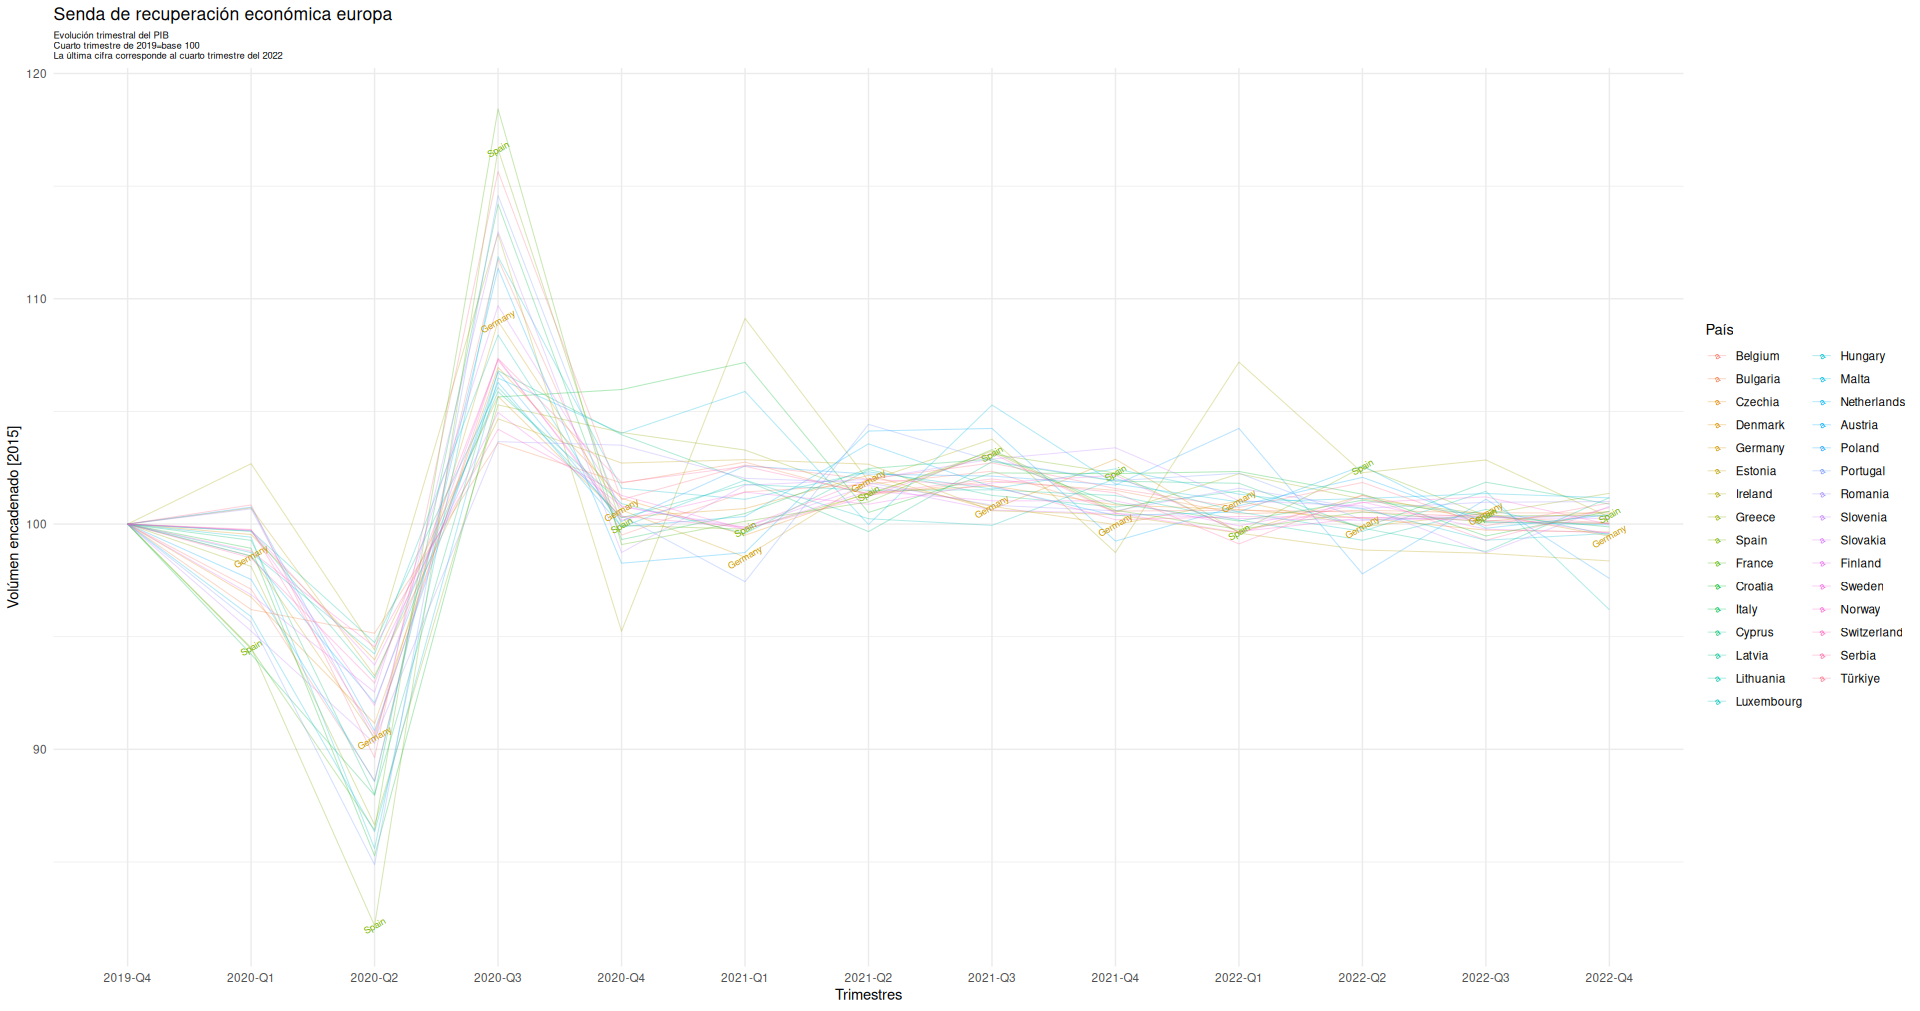
\includegraphics[scale=0.45,angle=90]{image/senda.png}

    %---------- EJERCICIO 7 -----------------
    \item Cada grupo deberá elegir una comunidad autónoma. Contabilidad Regional de España. Acceder a la información más reciente sobre el PIB por el lado de la demanda, la oferta y rentas. \\\\

    \begin{table}[htbp]
      \centering
      \caption{Producto interno bruto. OFERTA. Cataluña. 2022(p)}
      \vspace{0.3cm}
      \scalebox{0.5}{
	\begin{tabular}{l|rr}
	\toprule
	&Valor precios corrientes (M euros)&Variación en volumen (\%)\\
	\midrule
	    \textbf{PIB} &270710&5.5\\
			 Valor añadido bruto&250221&5.6\\
			 \quad Agricultura&1622&-13.9\\
			 \quad Industria&50186&-2\\
			 \qquad ind. manufacturera&39825&-1.5\\
			 \quad Construcción&11229&4.5\\
			 \quad Servicios&187185&7.9\\
			 \qquad Comercio, transporte, profesionales y otras&63430&14.6\\
			 \qquad Act. inmobiliarias, profesionales y otras&84067&6.5\\
			 \qquad Adm. pública, educación, sanidad y servicios sociales&39688&1.7\\
			 Impuestos netos sobre productos&20489&4.6\\
	\bottomrule
	\end{tabular}%
      \label{tab:addlabel}%
	}
      \begin{center}
      \tiny Fuente: Idescat.\\
      \tiny (p) = Datos provisionales.
      \end{center}
    \end{table}

    
    \begin{table}[htbp]
      \centering
      \caption{Producto interno bruto. DEMANDA. Cataluña. 2022(p)}
      \vspace{0.3cm}
      \scalebox{0.5}{
	\begin{tabular}{l|rr}
	\toprule
	&Valor precios corrientes (M euros)&Variación en volumen (\%)\\
	\midrule
	    \textbf{PIB}&270710&5.5\\
	    Demanda interna&232.794&3.2\\
	    \quad Consumo de los hogares&135491&4.1\\
	    Consumo de las adm. públicas (1)&46439&-0.1\\
	    \quad Formación bruta de capital (2)&50865&3.8\\
	    \qquad FBCF (bienes de equipo y otros activos)&26955&3.5\\
	    \qquad FBCF (construcción)&23231&4.8\\
	    Saldo exterior (3) (4)&37915&2.8\\
	    \quad Saldo con el extranjero (4)&20892&2.9\\
	    \qquad Exportaciones totales al extranjero&118322&14.0\\
	    \qquad \quad Exportaciones de bienes y servicios&103824&5.0\\
	    \qquad \quad Consumo de los extranjeros en el territorio&14498&162.8\\
	    \qquad Importaciones totales del extranjero&97430&7.5\\
	    \qquad \quad  Importaciones de bienes y servicios&93022&5.3\\
	    \qquad \quad Consumo de los residentes en el extranjero&4408&82.9\\
	\bottomrule
	\end{tabular}%
      \label{tab:addlabel}%
	}

	\footnotesize \tiny Fuente: Idescat.\\
	\footnotesize \tiny (1) Incluye el gasto en consumo de las instituciones sin finalidad de lucro al servicio de los hogares.\\
	\footnotesize \tiny (2) Incluye la formación bruta de capital fijo (FBCF) y la variación de existencias.\\
	\footnotesize \tiny (3) Incluye el saldo con el extranjero y con el resto de España.\\
	\footnotesize \tiny (4) La variación anual en volumen de los saldos se expresa como aportación al crecimiento del PIB.\\
	\footnotesize \tiny (p) Dato provisional.
    \end{table}


    \begin{table}[htbp]
      \centering
      \caption{Producto interno bruto. RENTAS. Cataluña. 2022(p)}
      \vspace{0.3cm}
      \scalebox{0.5}{
	\begin{tabular}{l|rr}
	\toprule
	&Valor precios corrientes (M euros)&Variación en volumen (\%)\\
	\midrule
	    \textbf{PIB} &270710&5.5\\
	    Remuneración de asalariados&270710&10.6\\
	    Excedente bruto de explotación &126807&6.9\\
	    Impuestos netos s/producción e Importación & 22664 & 5.1\\
	\bottomrule
	\end{tabular}%
      \label{tab:addlabel}%
	}
      \begin{center}
      \tiny Fuente: Idescat.\\
      \tiny (p) = Datos provisionales.
      \end{center}
    \end{table}


\end{enumerate}
